%%%%%%%%%%%%%%%%%%%%%%%%%%%%%%%%%%%%%%%%%%%%%%%%%%%%%%%%%%%%%%%%%%%%
%% appendix1.tex
%% UNL thesis document file
%%
%% Chapter with example of appendix with a short dummy text
%%%%%%%%%%%%%%%%%%%%%%%%%%%%%%%%%%%%%%%%%%%%%%%%%%%%%%%%%%%%%%%%%%%%
\chapter{Código da aplicação}
\label{cha:codigo_da_aplicacao}

\begin{figure}[hbtp]
	\centering
	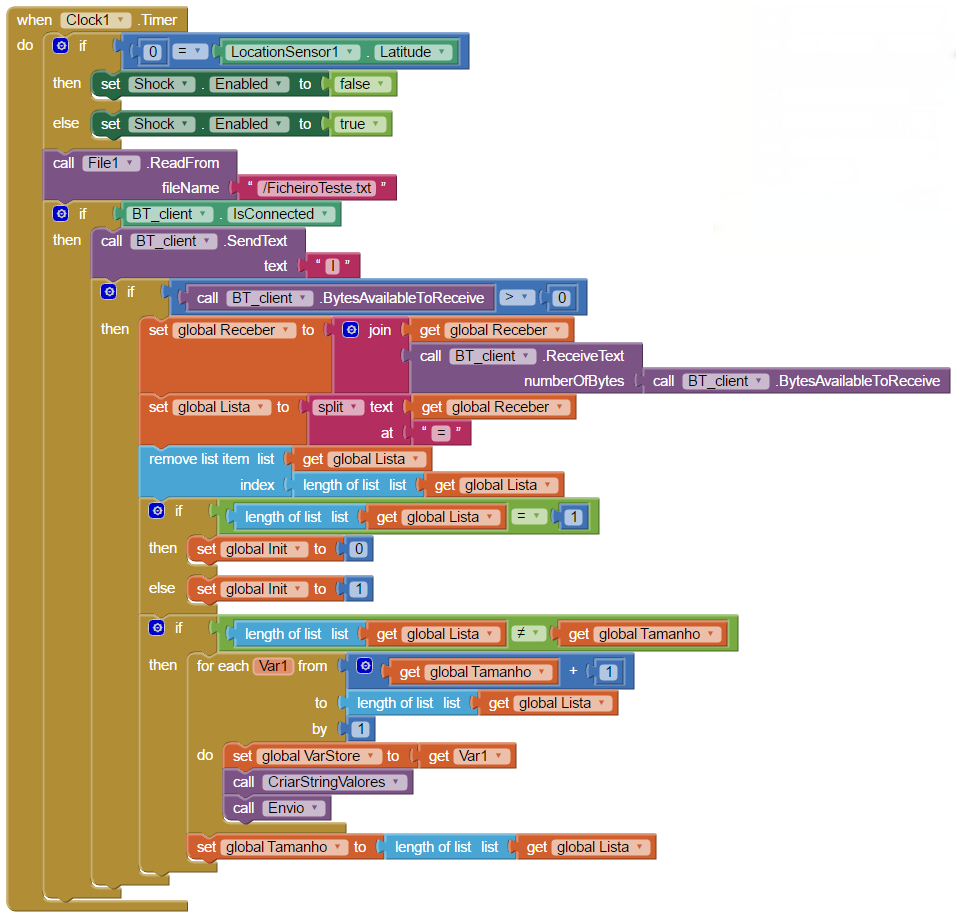
\includegraphics[width=14cm]{App4}
	\caption{Ciclo principal da aplicação}
	\label{fig:App4}
\end{figure}

\begin{figure}[hbtp]
	\centering
	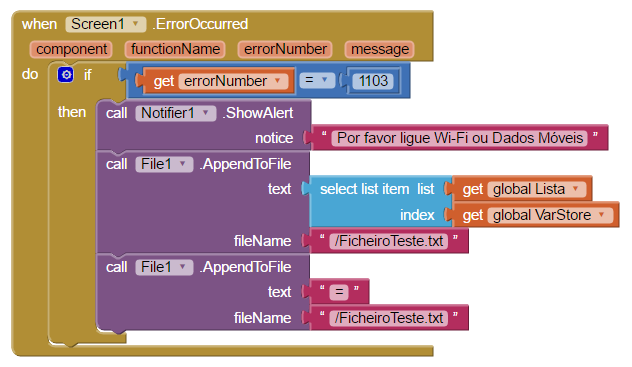
\includegraphics[width=14cm]{App6}
	\caption{Gestão de mensagens de erro}
	\label{fig:App6}
\end{figure}

\begin{figure}[hbtp]
	\centering
	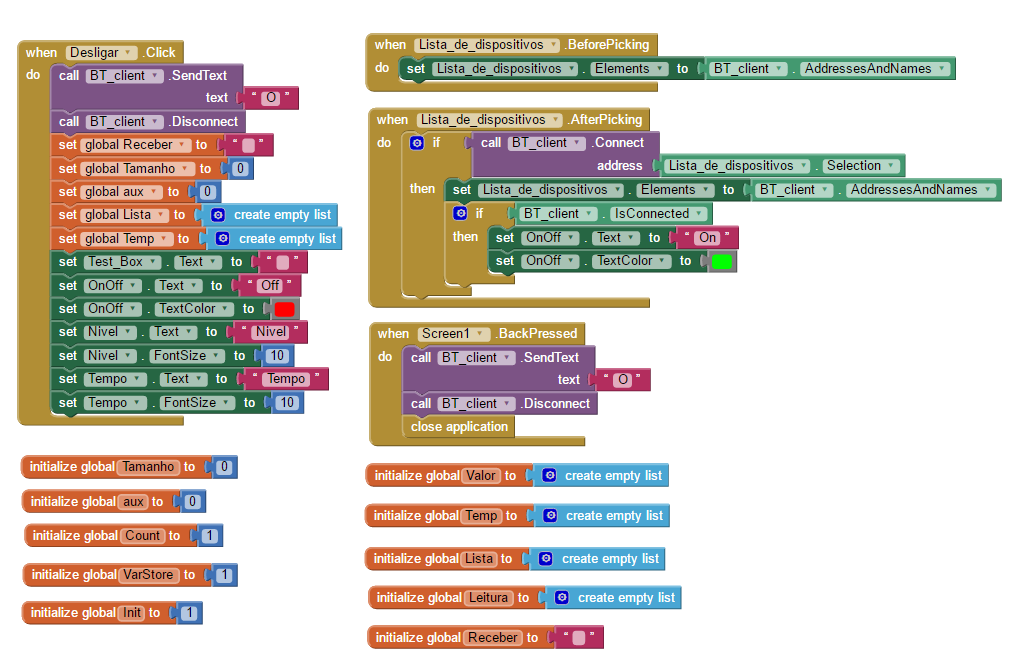
\includegraphics[width=14cm]{App1}
	\caption{Inicialização de variáveis e ações dos botões ``Desligar'' e ``Dispositivos''}
	\label{fig:App1}
\end{figure}

\begin{figure}[hbtp]
	\centering
	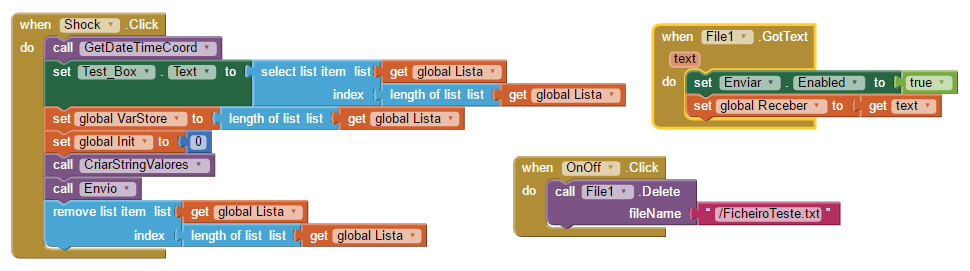
\includegraphics[width=14cm]{App2}
	\caption{Ação do botão ``Shock'' e remoção do ficheiro do telemóvel}
	\label{fig:App2}
\end{figure}

\begin{figure}[hbtp]
	\centering
	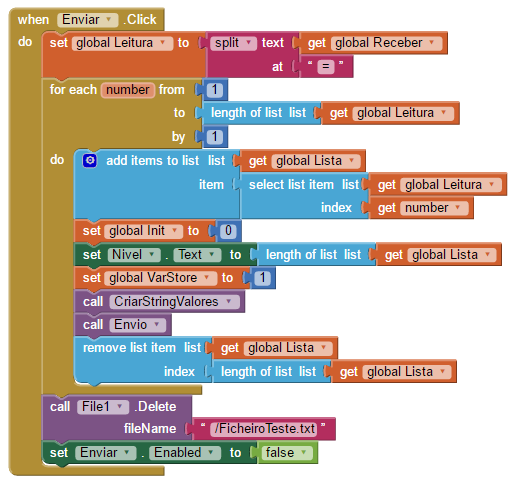
\includegraphics[width=14cm]{App3}
	\caption{Ação do botão ``Enviar''}
	\label{fig:App3}
\end{figure}



\begin{figure}[hbtp]
	\centering
	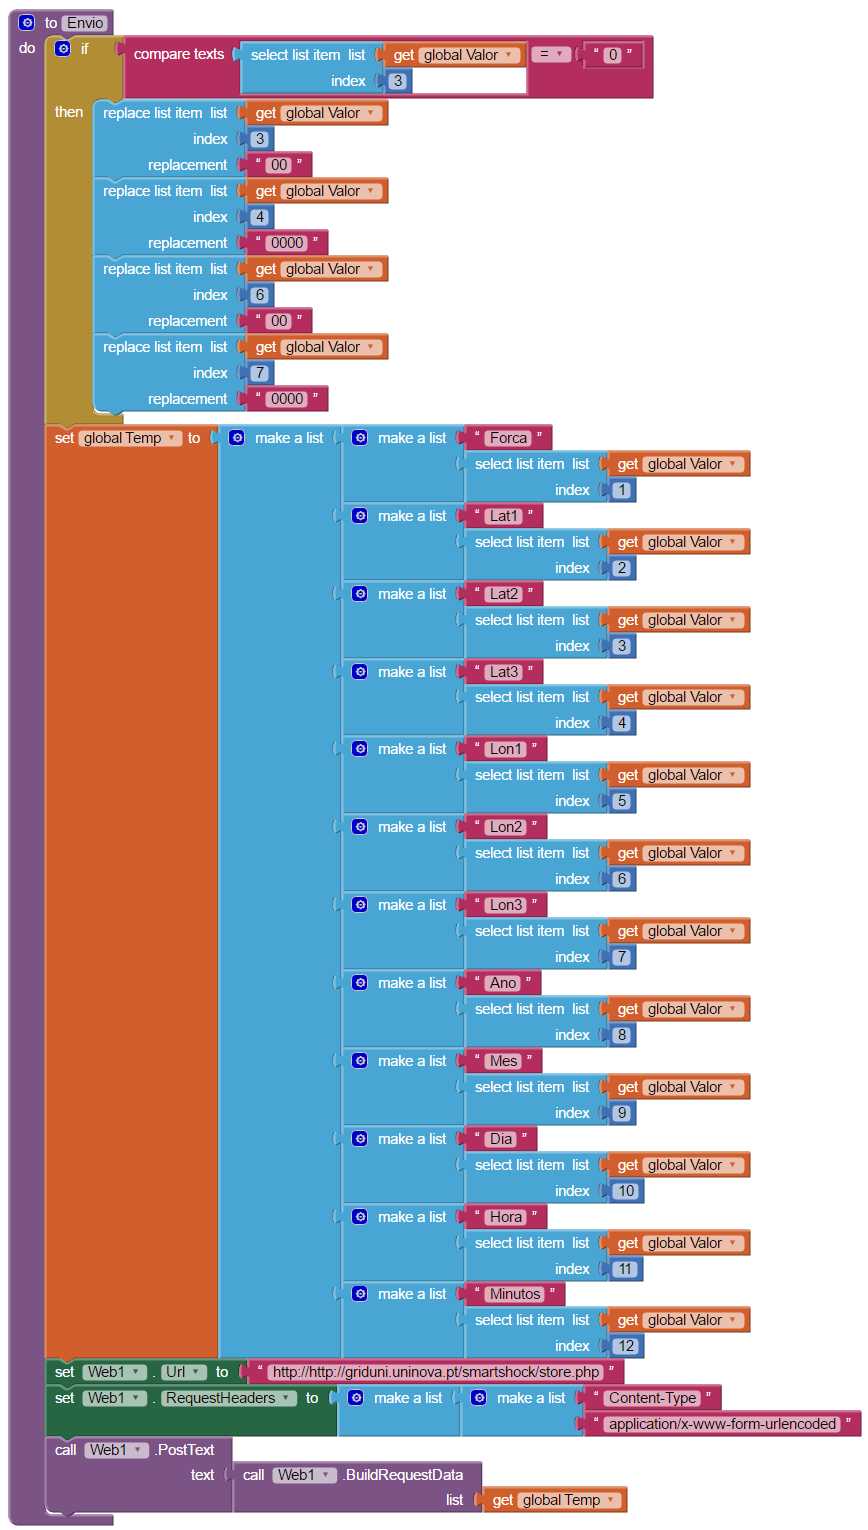
\includegraphics[width=14cm]{App5}
	\caption{Transformação de variáveis para envio para a base de dados}
	\label{fig:App5}
\end{figure}

